\chapter{Introduction}
L'étude du mouvement des corps humain et animal constitue un problématique à part entière pour l'ingénierie actuelle. En effet des nombreuses applications existent, qu'elles soient du domaine de l'imitation structurelle comme dans le milieux de la robotique par exemple, ou au contraire à des fin thérapeutiques à l'instar de l'ingénierie médicale.\\ 

\begin{figure}[h!]
    \centering
    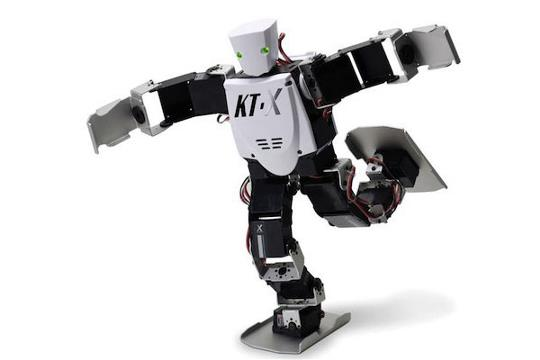
\includegraphics[scale = 0.4]{Images/Robot.jpg}
    \caption{Robovie-X Robot \cite{noauthor_robovie-x_nodate}}
    \label{figRobot}
\end{figure}

Si il y a plusieurs années les scientifiques devaient se contenter d'observations in vivo et de schéma structurels pour mettre aux points leur solutions, la possibilité de modéliser les corps sur ordinateur apporte un réel avantage à la recherche moderne, tant au médecin chirurgien ou orthopédique qu'à l'ingénieur. Ce dernier se vois d'ailleurs amené à travailler avec le corps médical pour arriver à adapter ses dispositifs théoriques sur un être vivant.\\

La spasticité est un symptôme musculaire d'origine neurologique dont soufre nombre de patients atteint notamment de sclérose en plaque. Cette affection provoque des trouble moteur aux niveau de jambes mais aussi au niveau des membres supérieurs les mettant dans l'incapacité de marcher et plus généralement de se mouvoir correctement.\\
Aujourd'hui des solution médicamenteuses et chirurgicales existent et certaines atèles proposent une correction du problème pour aider à la rééducation.\\

Ce stage se place dans un projet déjà débuté à l'ISIR sous la tutelle de M. Saint-Bauzel visant à réaliser un concept d'exosquelette qui aiderais à la rééducation en corrigeant les défauts de mouvement engendrés par des muscles spastiques.\\

Le travail présenté dans ce rapport couvre le premier problème auxquels tout concepteur d'un tel produit se trouveras forcément confronté : la simulation.\\ 
Il n'était pas question ici de réaliser un modèle d'assistance mais seulement de réaliser une première modélisation de ce que pourrait être le comportement d'un muscle spastique inséré dans le système locomoteur humain.\\ 
Dans un premier temps un travail bibliographique a été réalisé afin de se familiariser avec les différents modes de simulation musculaire. Le logiciel OpenSim a ensuite été pris en main et utiliser pour présenter un modèle musculaire à même d'intégrer une forme de spasticité.\\ Finalement des données comparatives entre différent modèles musculaires on été collectées et des procédures on été mise en place pour permettre une prise en main plus rapide du modèle déjà existant à l'avenir. 
